
\subsection{Data description}


\subsection{Estimation methodology}

\subsection{Abnormal returns in the market adjusted model}


\subsection{Short term abnormal returns in the Market Model}

To test hypothesis #1 and #2 of whether negative and positive SDG related events impacts firm value on the short term, we set apart negative and positive events and assess the aggregated development in abnormal returns 10 days before and 10 days after an event. Moreover, we isolate the effect of the individual SDGs to test hypothesis #4 of whether events on some sustainability goals are more relevant for investors than other. We apply the Market Model to measure abnormal returns around an event.   



\subsubsection{Negative news}

The average abnormal returns and development in cumulative average abnormal returns calculated from the Market Model are illustrated on aggregate in figure \ref{fig:ST_neg_news}. To support the analysis, the AAR and CAAR are portrayed along with their respective 95\% confidence intervals and the amount of events on a given day relative to the event date $(t = 0)$ (right y-axis) represented by the barplot in the background. 

The left y-axis depicts the abnormal return and the x-axis is the number of days before and after an event has occurred. The effect of negative events on average stock behavior is represented by the blue line in the graph, and is mostly negative leading up to an event. The impact from negative events is approximately zero until $t = -6$ upon which the AAR decreases steadily until the event date, where it bottoms at $-0.36\%$. After a negative event at $t=0$ the AAR increases, however still negative until $t=2$, towards neutrality at zero and remains there for the rest of the window. The CAAR stays negative during the full event window and bottoms on $t=2$ after a large decline of approximately $1.2\%$ from  $t=-5$. Moreover, the AAR is significantly negative between $t=-2$ and $t=0$ at $95\%$. The same goes for the CAAR after $t=-2$ and the remaining window. Generally, negative news seems to be priced in leading up to and including the identified event day, after which they have limited impact. \\ 
The bars offers insights into the extent of observations leading up to an event. The bars begin to increase at $t=-5$ at which the AAR begins to decline, which imply a relation between attention towards negative news and pessimistic investor behavior even before the event date. Furthermore, this is an indication that the specified event time may be lagging the incident of the *true* event, which is a disadvantage of this model setup. 

\begin{figure} [H]
    \centering
    \caption{Negative news: $CAAR_{t=10}$}
    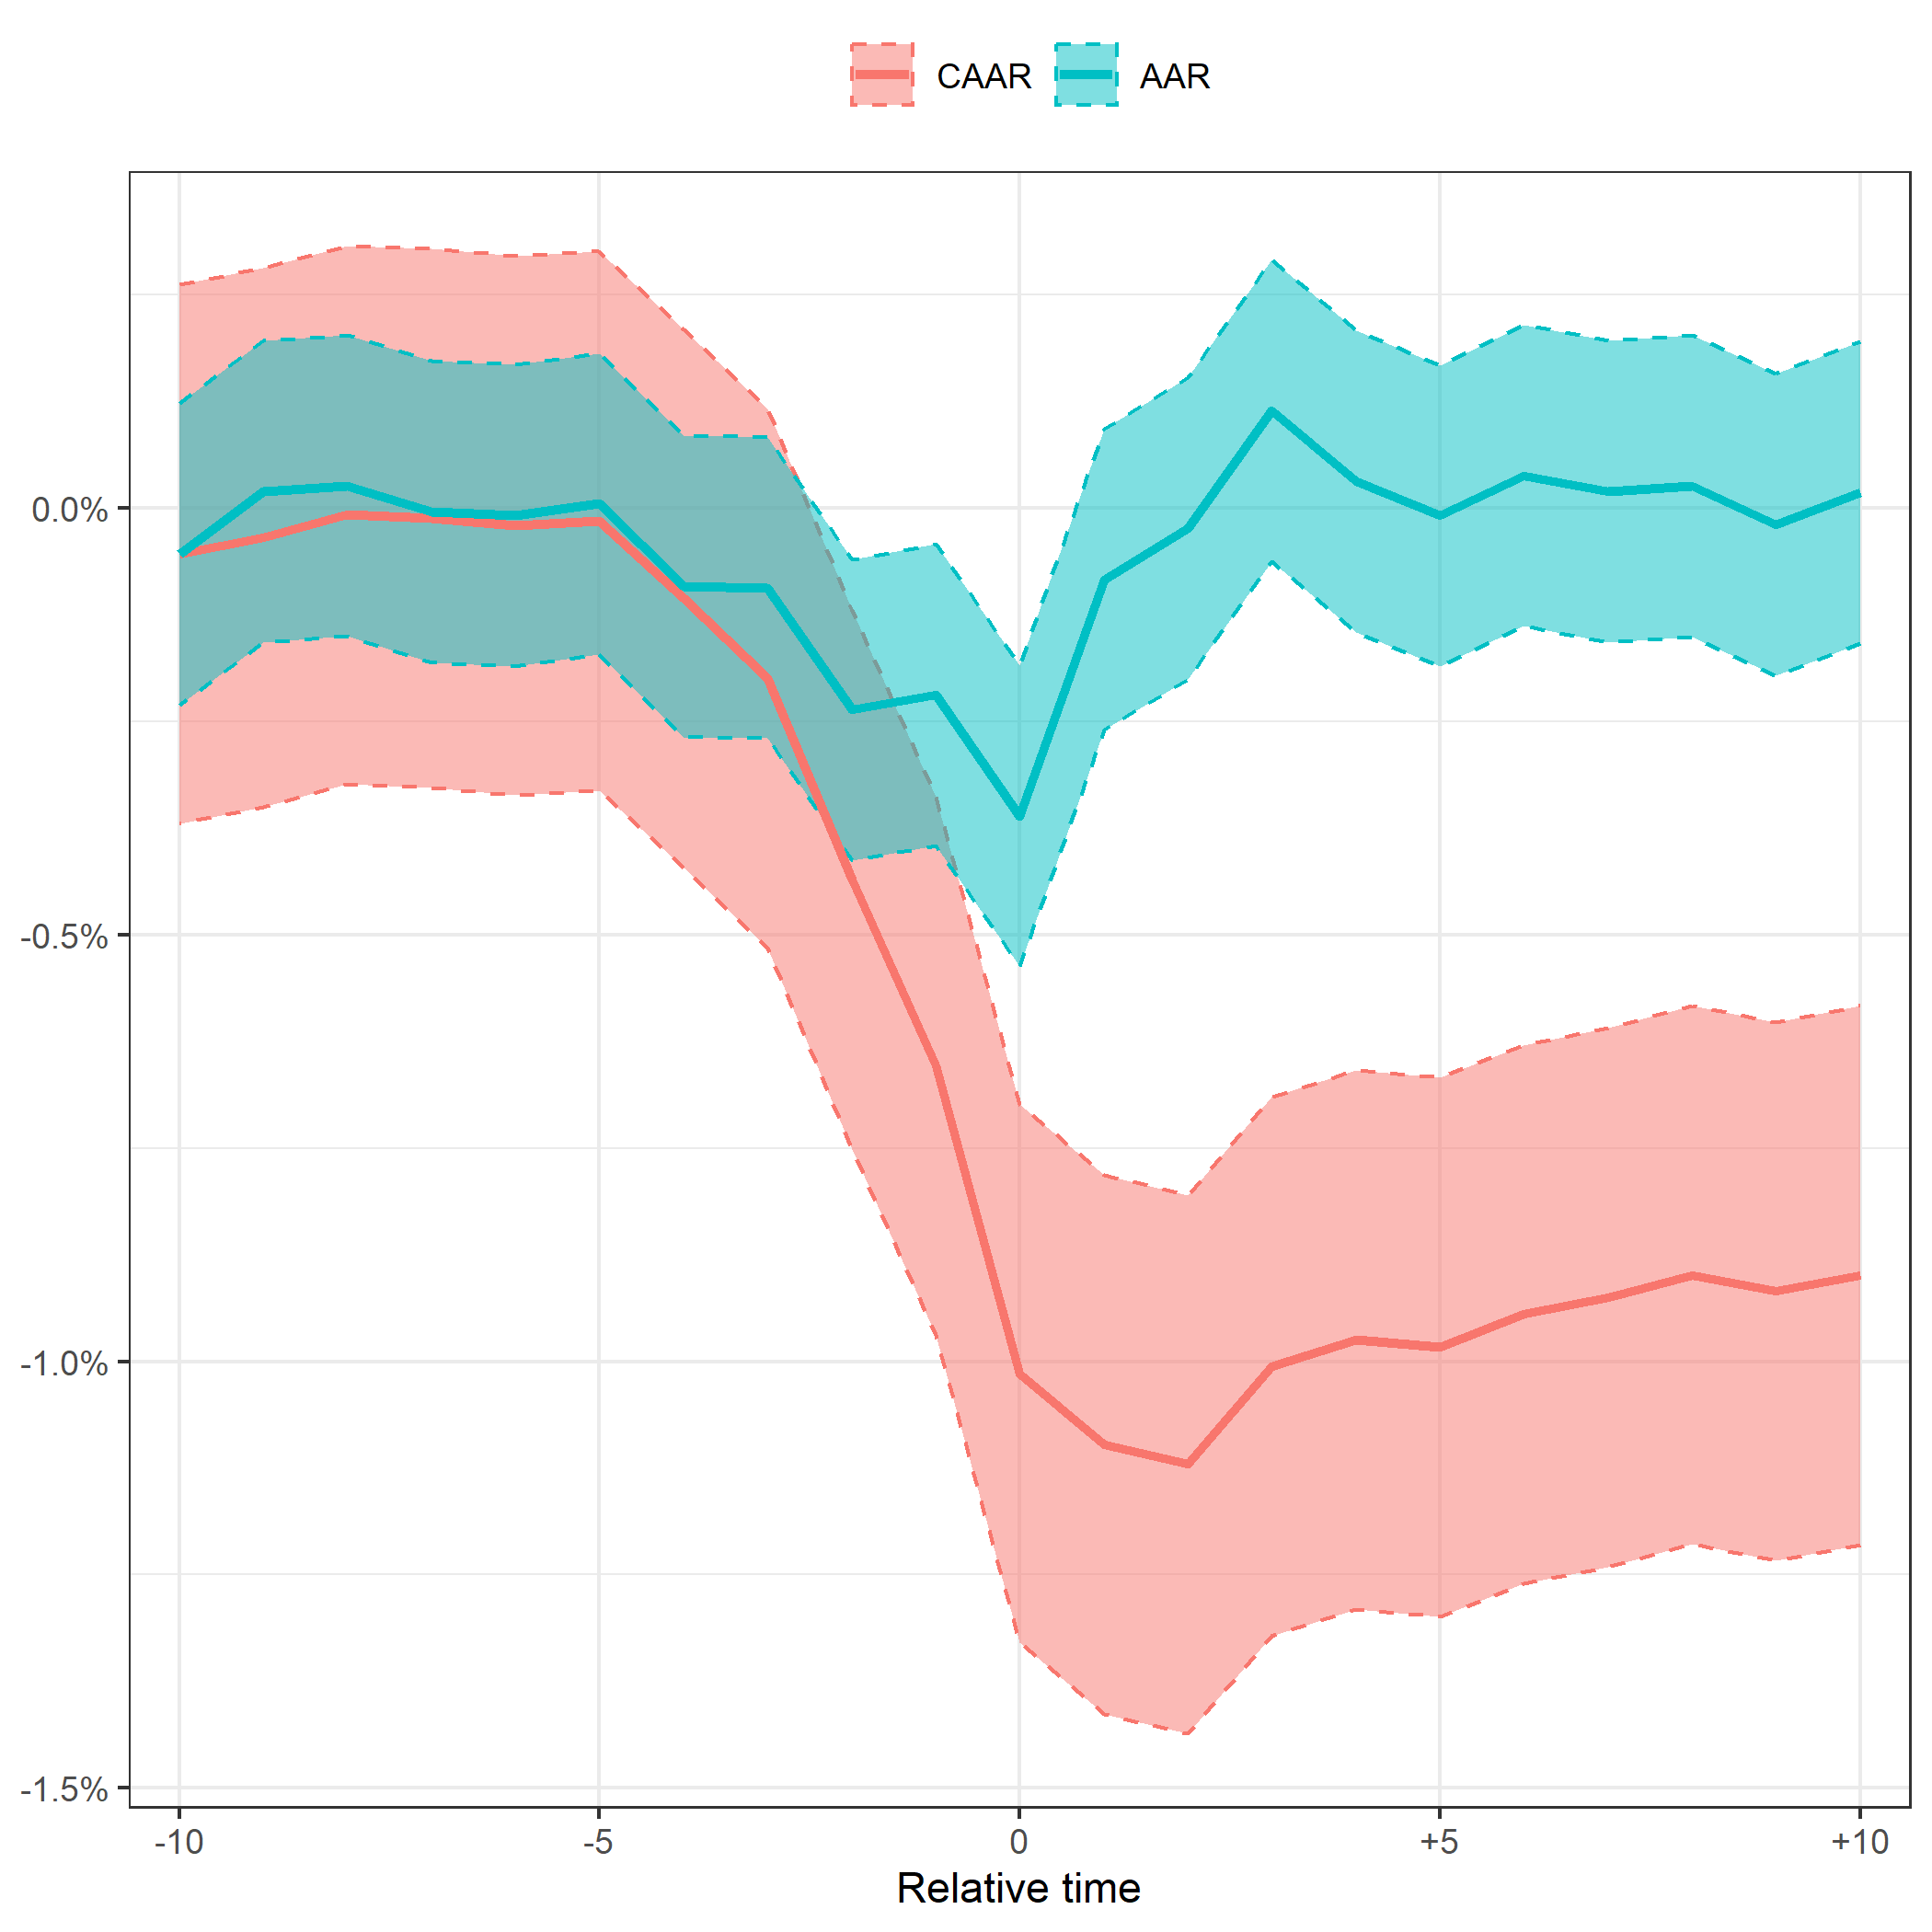
\includegraphics[scale=0.6]{Projekt/1.Figures analysis/ST_negative_all_CI.png}
     \caption*{\footnotesize The figure illustrates the average abnormal return (AAR) and cumulative AAR (CAAR) around the event date (t = 0) of negative news. The lines (left axis) represent the average and the ribbons represent the 95th confidence intervals. The bars (right axis) represent the amount of events on a given day relative to t = 0. }
    \label{fig:ST_neg_news}
\end{figure} 

Examining the average effect from, respectively, positive and negative events provides insights into the overall tendency of the relation between shareholder sentiment and corporate sustainability. By investigating the abnormal returns resulting from events specific to the individual SDGs one can gain a deeper understanding of which themes within corporate sustainability that investors places most emphasis with. Figure \ref{fig:ST_neg_bar} illustrates the aggregated CAAR over the full event window (from $t=-10$ to $t=10$) from events related to specific SDGs along with corresponding confidence intervals. 

\begin{figure} [H]
    \centering
    \caption{CAAR per SDG: Negative news}
    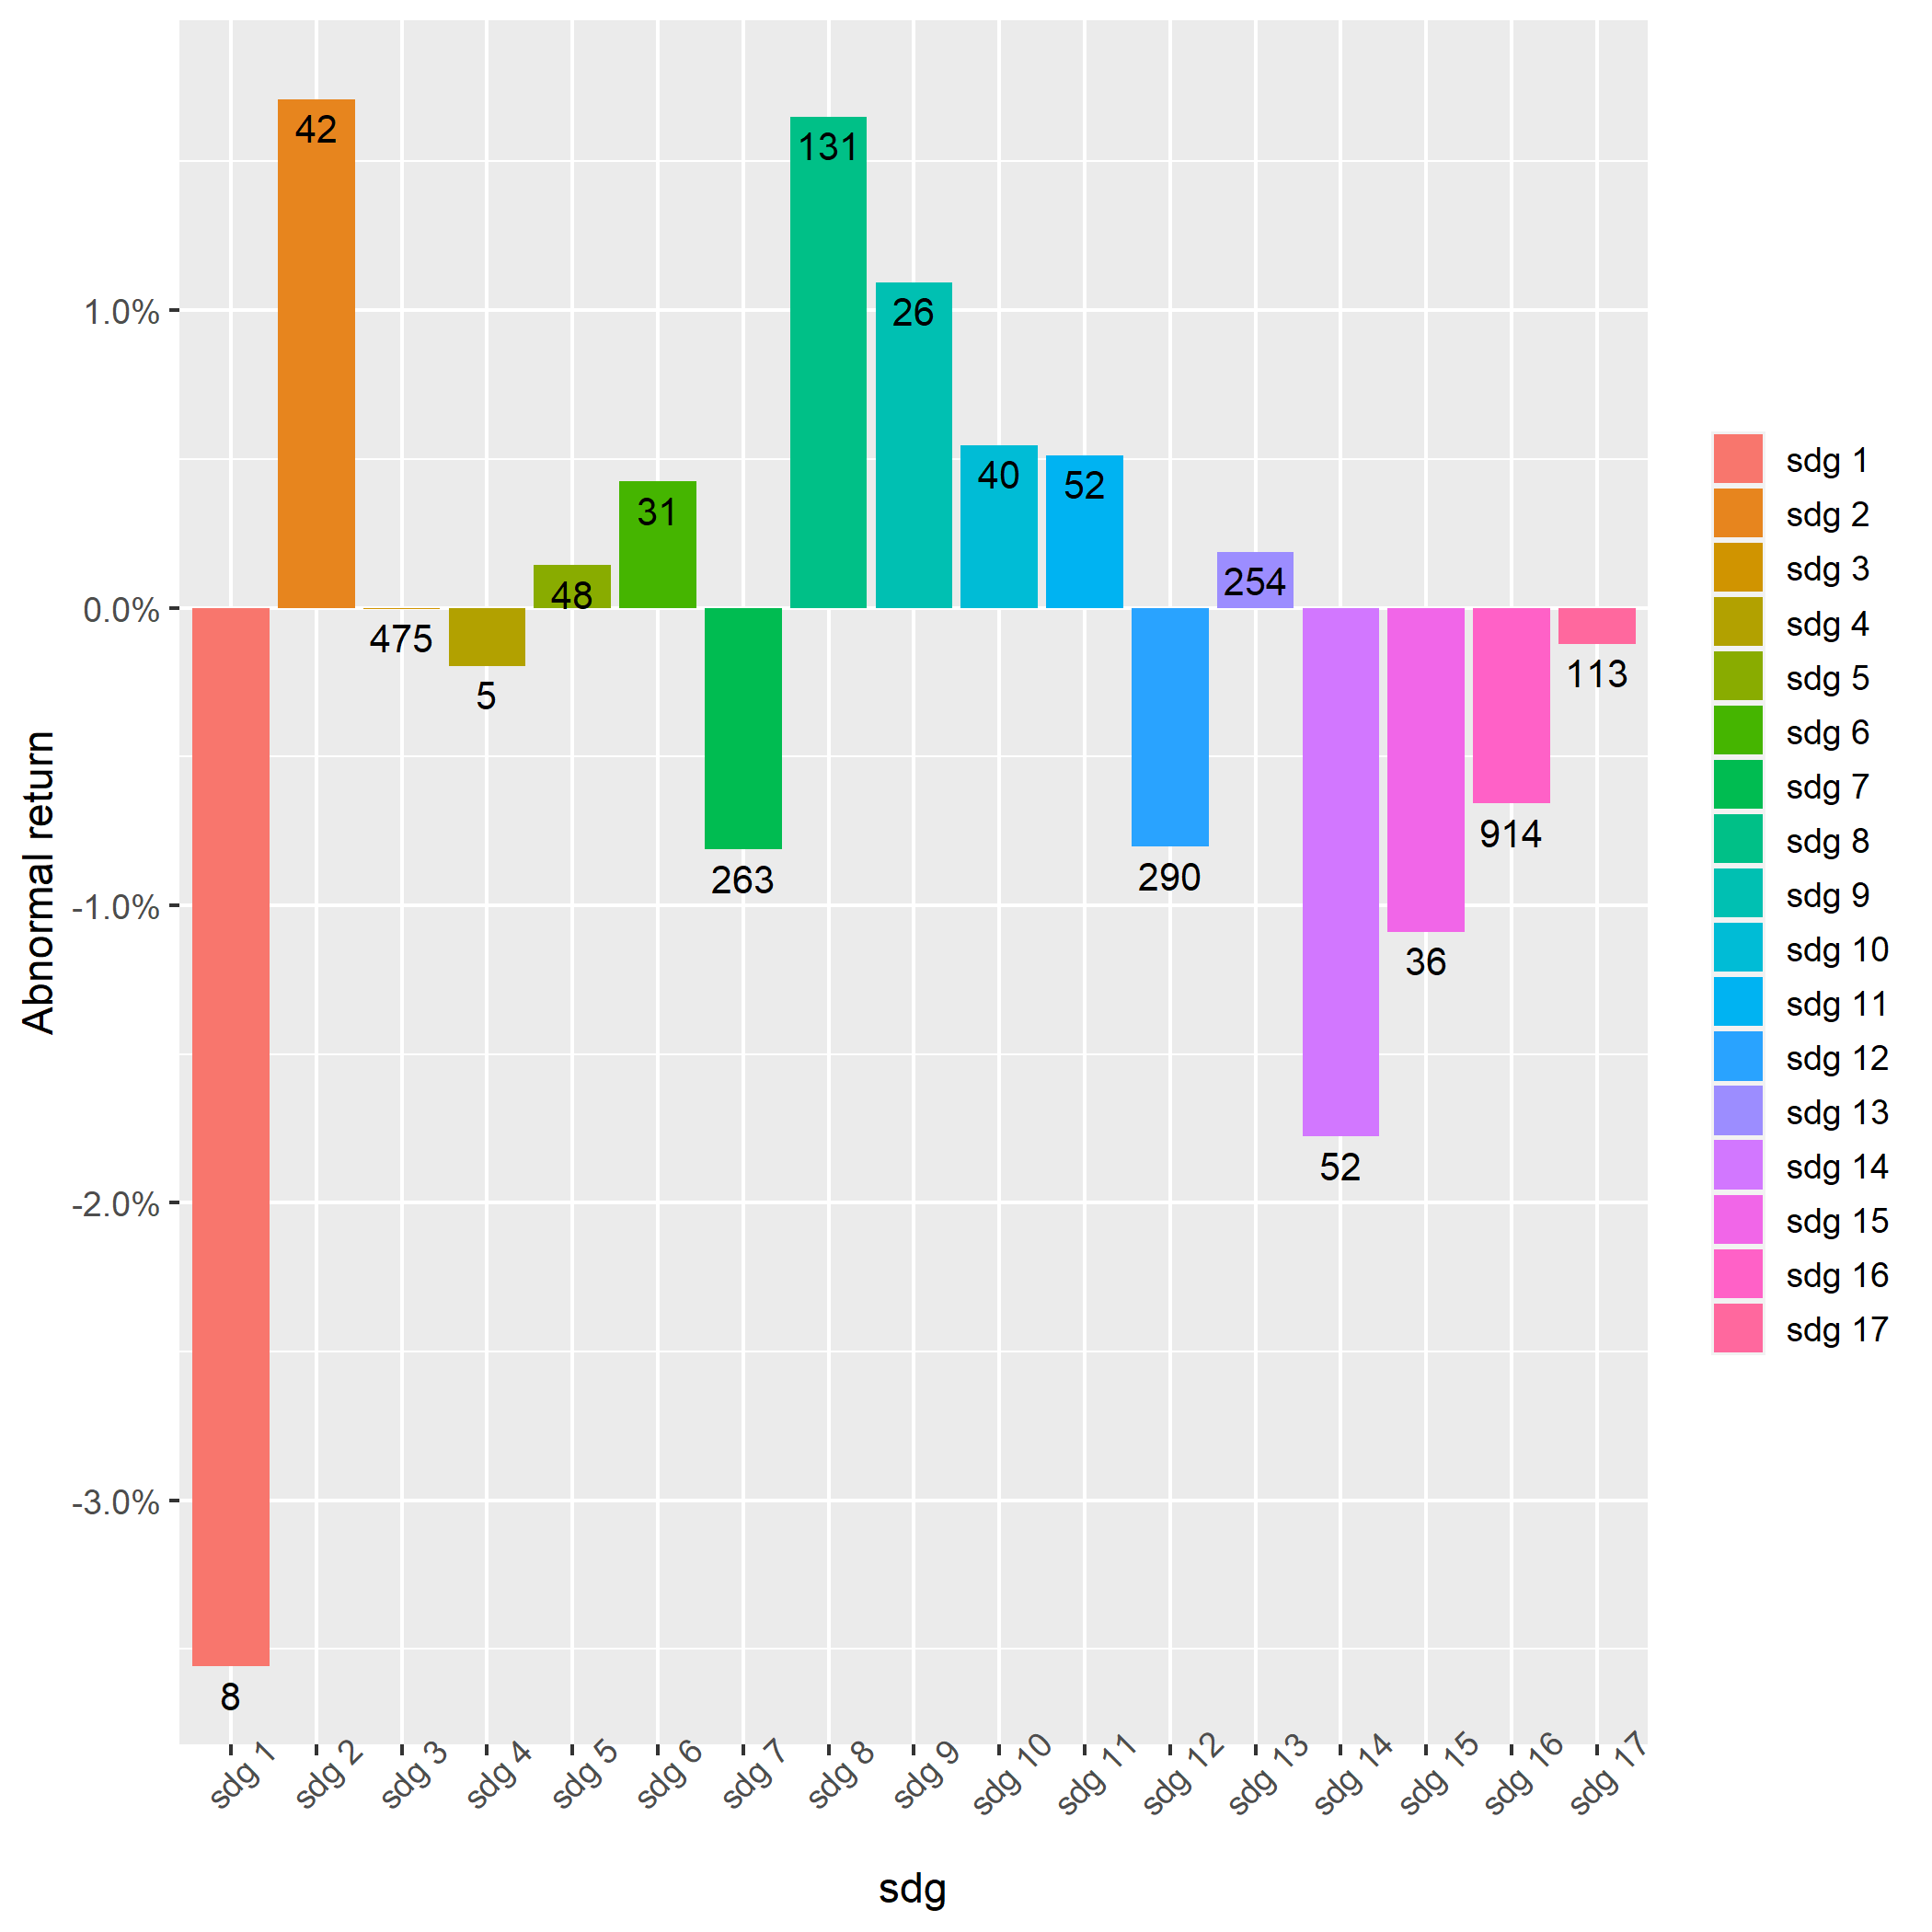
\includegraphics[scale=0.6]{Projekt/1.Figures analysis/ST_negative_sdg_bar.png}
    \caption*{\footnotesize The figure illustrates the CAAR on $t = 10$ (the full period) from negative news. The error bars represent the 95\% confidence intervals of the CAAR.}
    \label{fig:ST_neg_bar}
\end{figure}

Splitting the events on SDGs generally illustrate that negative events in most groups are associated with negative abnormal returns. However, the issue of statistical uncertainty in the measurements means that one cannot generate a lot of insights from the aggregated values. Only SDG 15 and 16 provides abnormal returns significantly different from zero. The statistical uncertainty originates from the relatively low amount of observations associated with the individual groups after dividing the events into SDGs. For example, SDG 4 and 9 has only, respectively, 16 and 83 observations, which results in a vast excessively wide confidence interval, whereas SDG 12 and 16 has, respectively, 576 and 1364 observations, and correspondingly very narrow error bands. 

The significance of the results in relation to negative and positive events are summarised with a z-test in table \ref{tab: ST_significace}, which presents the z-scores and significance complementary to the AAR on $t=0$, along with the CAAR on respectively, two, five, and 10 days around the event.  



The selection method for negative events was proposed to gather cases of severe negative abnormal returns. The CAAR of the full and subset windows from negative events are significantly different from zero at $p \; < 0.01$, which further validates the selection method and that negative abnormal returns are attainable to negative events. However, the method may be late to pick up the signal of negative events or new information on the market.  

\begin{table}[ht]
\centering
\caption{AAR and CAAR over event window (in percentage)} 
\begin{tabular}{lllll}
   \hline  \hline
  & $AAR_{t=0}$ & $CAAR_{[-2;+2]}$ & $CAAR_{[-5;+5]}$ & $CAAR_{[-10;+10]}$  \\
 \hline
Positive news & $\underset{(1.973)^{**}}{0.073}$  & $\underset{(-0.211)}{-0.016}$    & $\underset{(-0.379)}{-0.043}$ & $\underset{(-1.091)}{-0.164}$  \\ 
Negative news & $\underset{(-3.457)^{***}}{-0.360}$  & $\underset{(-5.749)^{***}}{-0.917}$    & $\underset{(-4.761)^{***}}{-0.955}$ & $\underset{(-3.288)^{***}}{-0.888}$  \\ 
   \hline
   \multicolumn{5}{p{12cm}}{\footnotesize  $^* \; p\; <\; 0.1$, $ ^{**} \; p\; <\; 0.05$, $ ^{***} \; p\; <\; 0.01$  } \\ 
\end{tabular}
\label{tab: ST_significace}
\end{table}

\subsubsection{Positive news}

According to figure \ref{fig:ST_pos_news} the identified positive events doesn't seem to be associated with any significant reaction from the shareholders on average, as the AAR doesn't fluctuate significantly from zero during the event window besides a marginal deviation at the event date. Following, the statistical uncertainty of the CAAR becomes more widespread through the event window, as indicated by the widening red ribbon. The negative tendency of the CAAR is insignificant since the measure is based on, likewise, insignificant AARs, meaning that one cannot for certain state that the cumulative effect is different from zero. 

\begin{figure} [H] 
    \centering
    \caption{Short term positive news: AAR and CAAR}
    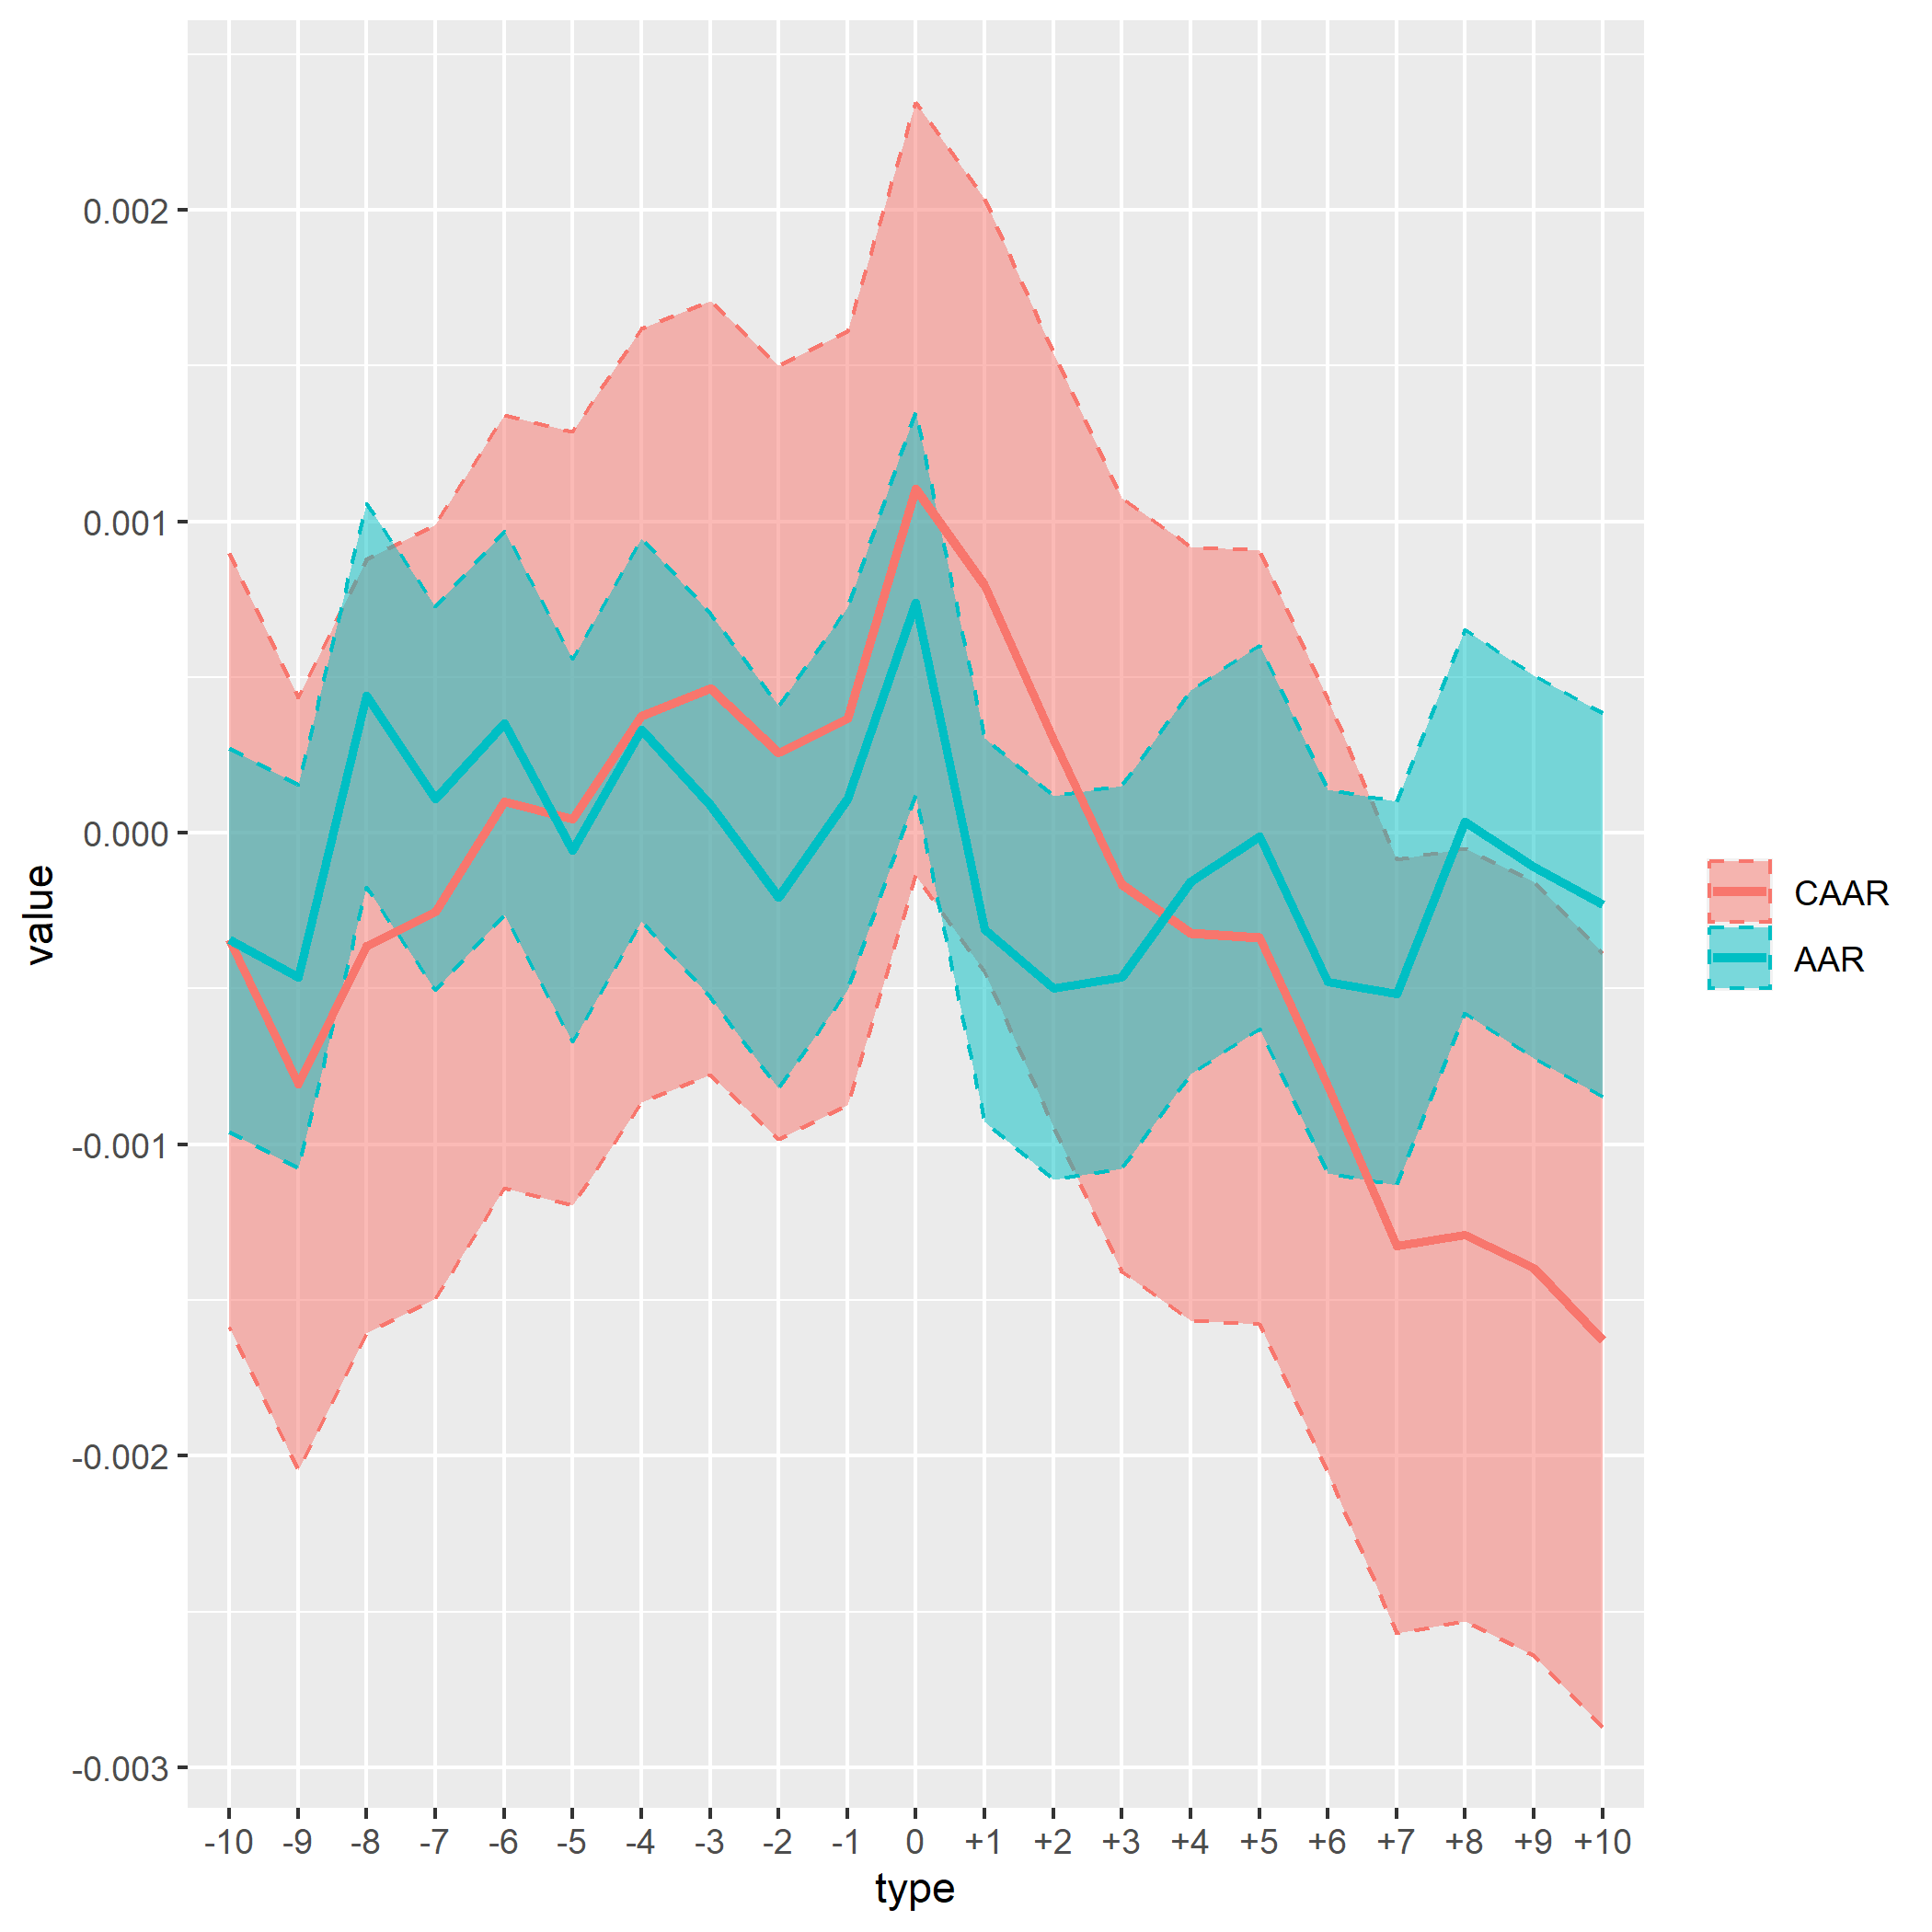
\includegraphics[scale=0.6]{Projekt/1.Figures analysis/ST_positive_all_CI.png}
    \caption*{\footnotesize The figure illustrates the average abnormal return (AAR) and cumulative AAR (CAAR) around the event date (t = 0) of positive news. The lines (left axis) represent the average and the ribbons represent the 95th confidence intervals. The bars (right axis) represent the amount of events on a given day relative to t = 0. }
    \label{fig:ST_pos_news}
\end{figure}


The tendency of insignificance related to positive events is further reinforced by the results from the individual SDGs, as most are statistically indistinguishable from zero. However, the aggregates do indicate that positive events on SDGs in general are associated with negative abnormal returns. In contrast to the case of negative events, where the main issue was the amount of observations, the underlying issue with uncertainty comes with the seemingly random shareholder reaction to positive events. 
 
\begin{figure} [H]
    \centering
    \caption{CAAR per SDG: Positive news}
    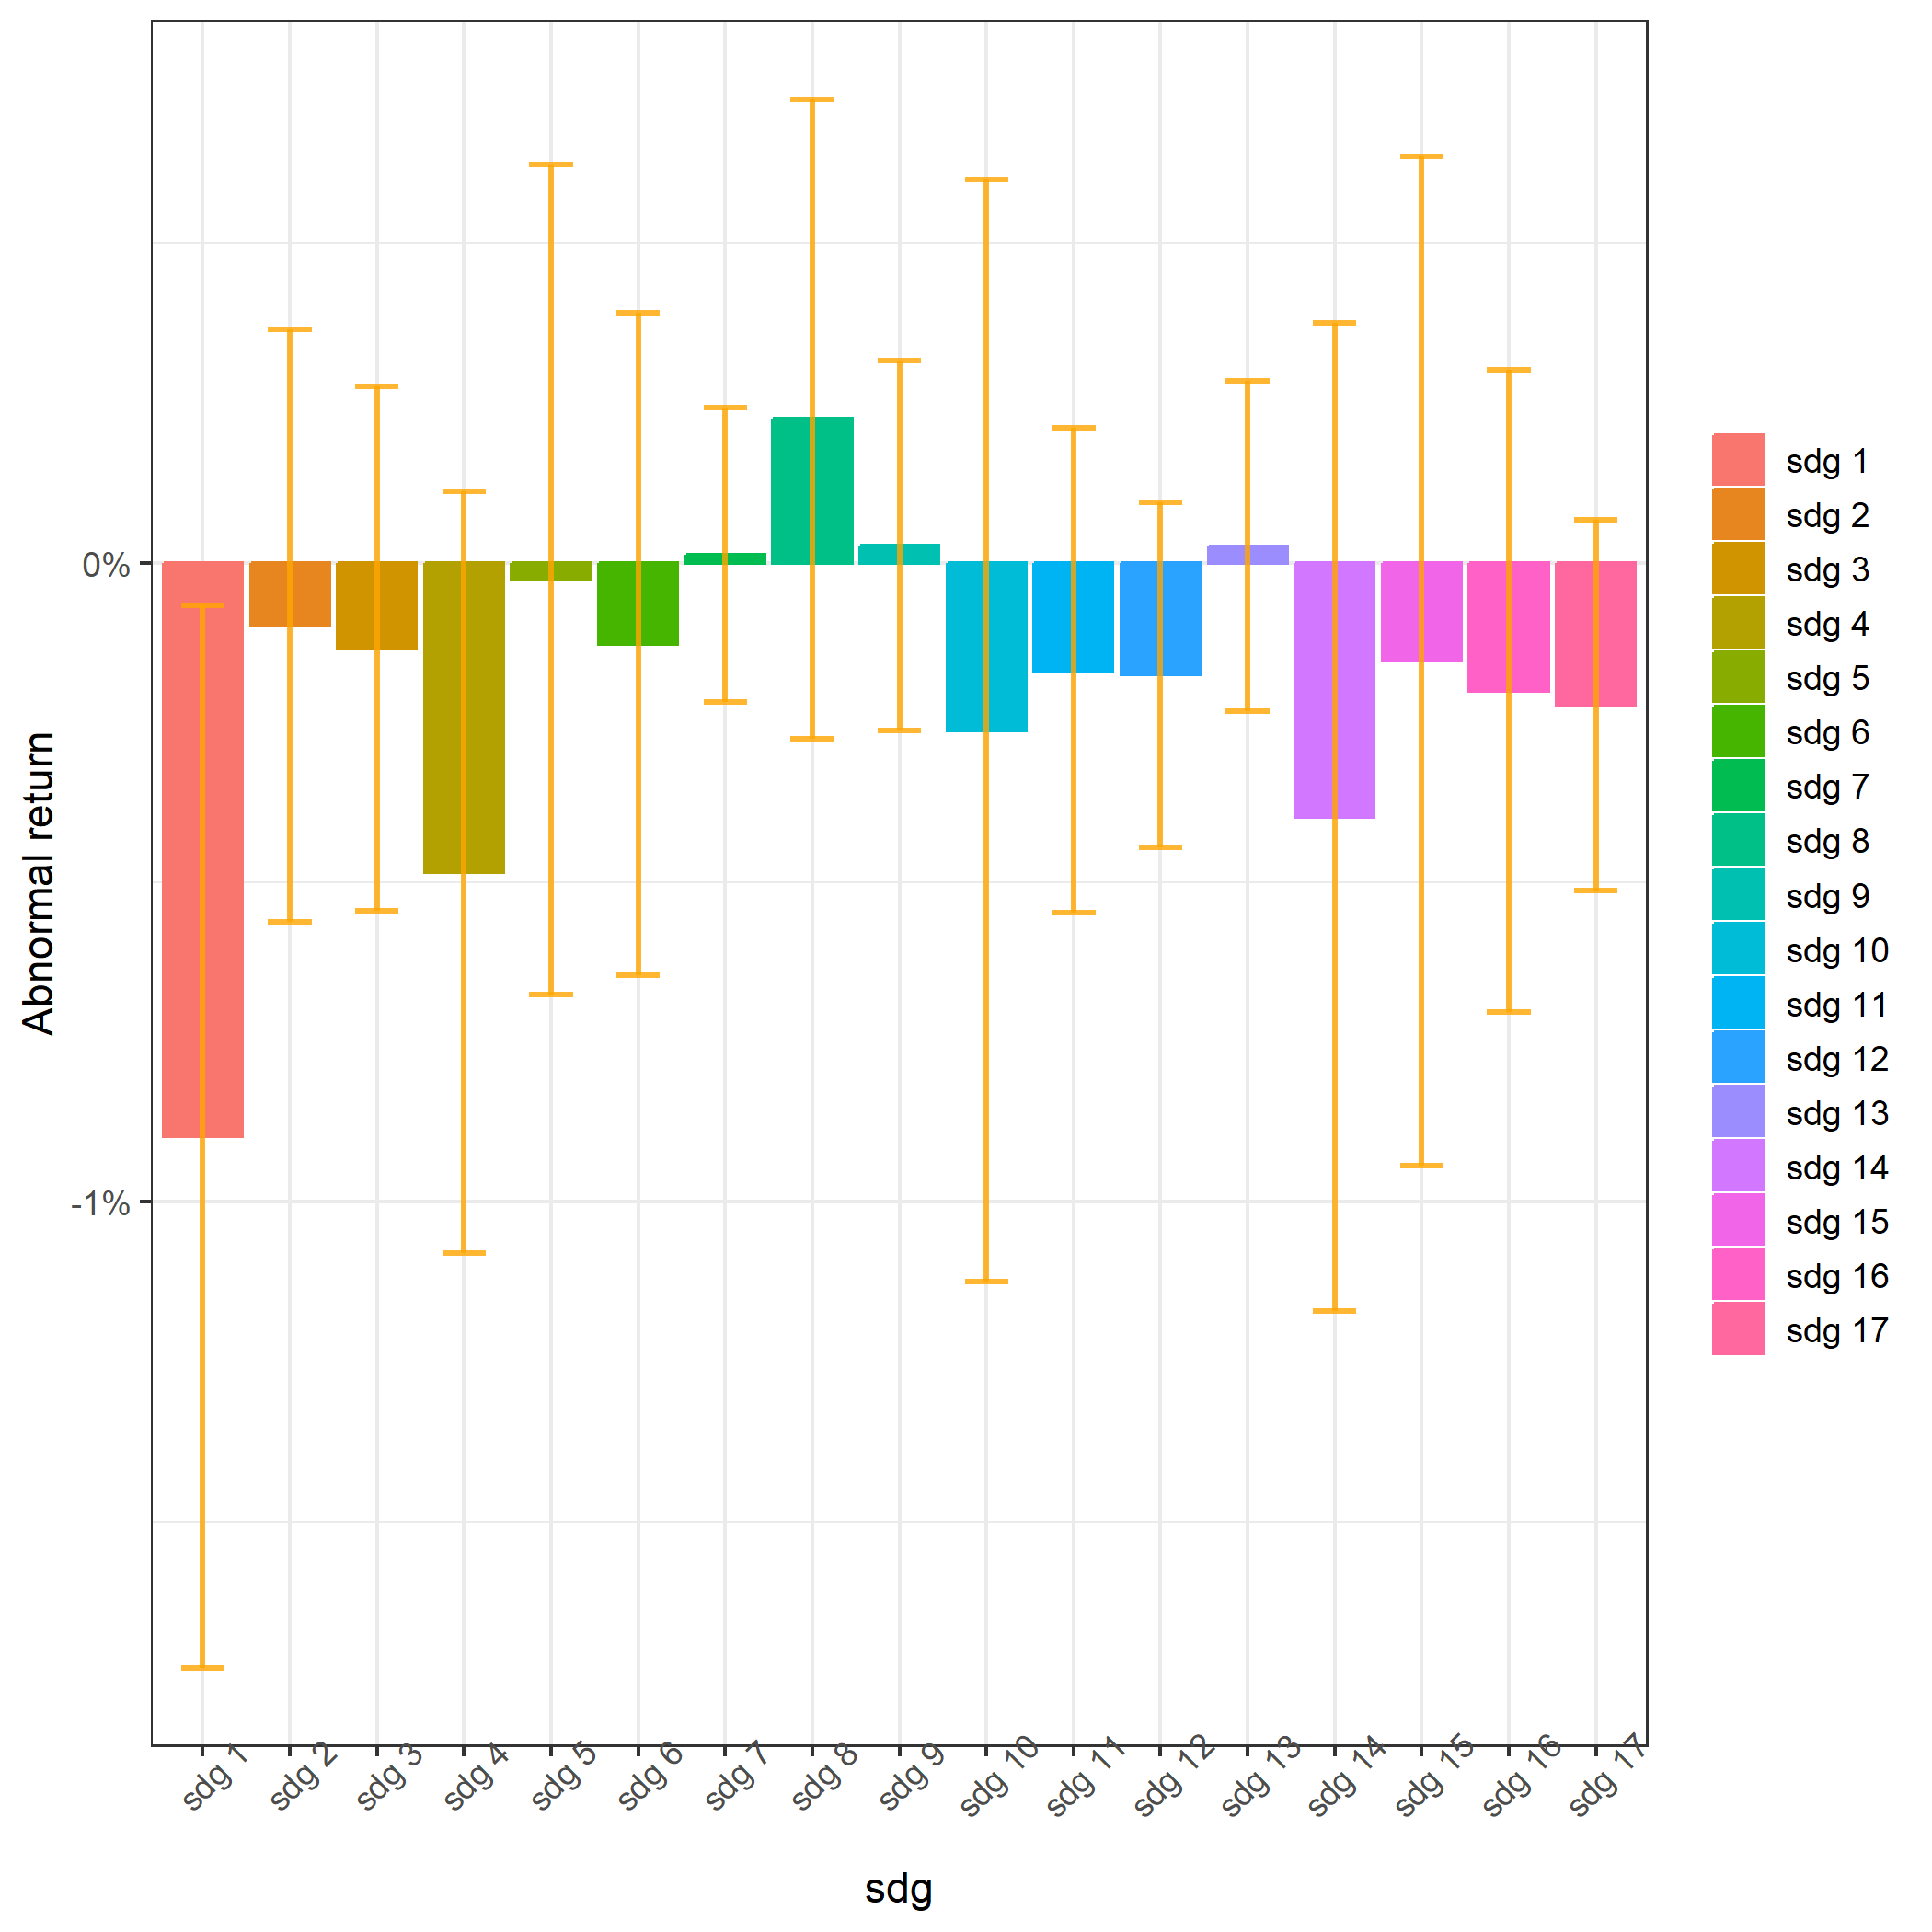
\includegraphics[scale=0.6]{Projekt/1.Figures analysis/ST_positive_sdg_bar.png}
    \caption*{\footnotesize The figure illustrates the CAAR on $t = 10$ (full period) from positive news. The error bars represent the 95\% confidence intervals of the CAAR.}
    \label{fig:ST_pos_bar}
\end{figure}

The insignificance of the abnormal returns associated with positive events are manifested in table \ref{tab: ST_significace}. The the CAARs on, respectively, two, five and 10 days around the event are all insignificantly different from zero. In contrast the AAR exhibit positive performance at $t = 0$ at 5\% significance. 

Generally, the short term empirical evidence demonstrate a non-verifiable relation between positive events, related to both broad and specific SDGs, and abnormal returns. Positive news is however associated with an instant reaction from investors on the event date. The evidence point towards an overall negative relationship, but this is not statistically valid.  


\subsection{Long term abnormal returns}


